\documentclass[report,gutter=10mm,fore-edge=10mm,uplatex,dvipdfmx]{jlreq}

\usepackage{lmodern}
\usepackage{amssymb,amsmath}
\usepackage{ifxetex,ifluatex}
\usepackage{actuarialsymbol}
\usepackage[]{natbib}
\RequirePackage{plautopatch}

% maru suji ① etc.
\usepackage{tikz}
\newcommand{\cir}[1]{\tikz[baseline]{%
\node[anchor=base, draw, circle, inner sep=0, minimum width=1.2em]{#1};}}

\usepackage{comment}

\begin{comment}

\ifnum0\ifxetex1\fi\ifluatex1\fi=0 % if pdftex
  \usepackage[T1]{fontenc}
  \usepackage[utf8]{inputenc}
  \usepackage{textcomp} % provide euro and other symbols
\else % if luatex or xetex
  \usepackage{unicode-math}
  \defaultfontfeatures{Scale=MatchLowercase}
  \defaultfontfeatures[\rmfamily]{Ligatures=TeX,Scale=1}
\fi
% Use upquote if available, for straight quotes in verbatim environments
\IfFileExists{upquote.sty}{\usepackage{upquote}}{}
\IfFileExists{microtype.sty}{% use microtype if available
  \usepackage[]{microtype}
  \UseMicrotypeSet[protrusion]{basicmath} % disable protrusion for tt fonts
}{}
\makeatletter
\@ifundefined{KOMAClassName}{% if non-KOMA class
  \IfFileExists{parskip.sty}{%
    \usepackage{parskip}
  }{% else
    \setlength{\parindent}{0pt}
    \setlength{\parskip}{6pt plus 2pt minus 1pt}}
}{% if KOMA class
  \KOMAoptions{parskip=half}}
\makeatother
\usepackage{xcolor}
\IfFileExists{xurl.sty}{\usepackage{xurl}}{} % add URL line breaks if available
\IfFileExists{bookmark.sty}{\usepackage{bookmark}}{\usepackage{hyperref}}
\hypersetup{
  hidelinks,
  pdfcreator={LaTeX via pandoc}}
\urlstyle{same} % disable monospaced font for URLs
\usepackage{longtable,booktabs}
% Correct order of tables after \paragraph or \subparagraph
\usepackage{etoolbox}
\makeatletter
\patchcmd\longtable{\par}{\if@noskipsec\mbox{}\fi\par}{}{}
\makeatother
% Allow footnotes in longtable head/foot
\IfFileExists{footnotehyper.sty}{\usepackage{footnotehyper}}{\usepackage{footnote}}

\end{comment}
%\makesavenoteenv{longtable}
\setlength{\emergencystretch}{3em} % prevent overfull lines
\providecommand{\tightlist}{%
  \setlength{\itemsep}{0pt}\setlength{\parskip}{0pt}}
\setcounter{secnumdepth}{-\maxdimen} % remove section numbering

\author{kazuyoshi}
\date{}

\newcommand{\problem}[1]{\subsubsection{#1}\setcounter{equation}{0}}
%\newcommand{\answer}[1]{\subsubsection{#1}}
\newcommand{\answer}[1]{\subsubsection{解答}}

%Pdf%\newcommand{\wakumaru}[1]{\framebox[3zw]{#1}}
\newcommand{\wakumaru}[1]{#1}






\begin{document}
\chapter{保険1第2章 解約および解約返戻金}
\section{2.2 解約および解約返戻金の意義と法規整}
\problem{H20 生保1問題 1(3)}
「保険料計算基礎率」と「責任準備金計算基礎率」が異なっている場合において、「解約返戻金計算基礎率」の設定方法について説明しなさい。
\answer{解答}
解約返戻金計算基礎率は、以下の観点から、保険料計算基礎率と同じに設定することが考えられる。  
\begin{itemize}
\item 解約返戻金は、個々の契約者が会社財産の形成に貢献した金額を基準とするものであ  り、契約者が拠出した金額は保険料であることから、解約返戻金の算定は保険料に基づくことが整合的である。
\item 一方、責任準備金は、ソルベンシーを考慮して会社が評価し積み立てるものであり、契約者価額ではない。
\item 補完的な観点として、解約返戻金水準は契約時に約定が必要であるが、責任準備金は経済状況等により保険期間途中でも積み増しまたは削減があり得る。それをこうした約定に反映することは困難である。
\end{itemize}

\section{2.3 解約控除の理由}

\problem{H4 生保1問題 1(2)}
解約控除について簡潔に説明せよ。
\answer{解答}
責任準備金に控除率を適用して解約返戻金を算出する場合に、その控除を解約控除という。
解約控除の理由としては、
\begin{itemize}
\item 新契約費の回収、
\item 解約による逆選択の防止と被保険群団の維持、
\item 解約に手間がかかる、
\item 投資上の不利益、
\item 数学的危険の不安定さの増加等が挙げられる。
\end{itemize}

\problem{H14 生保1問題 1(5)、H11 生保1問題 2(2)①}
個人保険・個人年金保険において解約控除を行う理由を列挙し簡潔に説明せよ。
\answer{解答}
解約控除の理由としては一般的に次の4つの理由が挙げられる。
\begin{enumerate}
\item 新契約費の回収:新契約時にかかる生命保険の募集・締結のための経費は、営業保険料中に予定事業費として組み込んでいる。保険契約が解約された場合には以後の保険料が回収
  されず新契約費はすでに支出されている一方で、その財源である予定新契約費(保険料)の収入が完結していないことになる。このため、未回収部分(の一部)を解約返戻金の算式に反映するものである。
\item 逆選択防止:一般に保険契約を解約する者は平均的に健康体であることが想定され、残された保険群団の死亡率が高まることが予想される。このため、残された保険群団の収支悪化を補うものである。
\item 投資上の不利益:解約を見込んで資産の流動性を図ることになるが、このことが資産運用利回りを低下させるため、これを補うものである。
\item ペナルティー:解約に伴う上記の様々な不利益へのペナルティーという意味合いである。
\end{enumerate}

\section{2.4 解約返戻金に関する視点}

\problem{H21 生保1問題 2(2)改}
個人保険の解約返戻金を決めるにあたって考慮すべき視点を5つ\footnote{元の問題は4つ. H21以降で、教科書の改定で「収益性」の追加があったのかも? }挙げ、それぞれ簡潔に説明しなさい。
\answer{解答}
\begin{enumerate}
\item 健全性
  \begin{itemize}
  \item 解約者に対して解約返戻金を支払うことは、保険群団に留保される金額、すなわち将来の保険債務に備えるための責任準備金積立財源となるものが少なくなるということである。
  \item このため、保険群団としての健全性の観点から、解約返戻金は、必要な責任準備金、及びソルベンシーマージンの積立財源を脅かさない金額以下で設定する必要があり、
  \item 具体的には少なくとも、解約返戻金は責任準備金額以下とすべきである。
  \item いわゆる「解約控除」は、健全性の視点で設定していると見ることもでき、
  \item 残存契約からの収益に期待せずに、新契約費の未回収部分を賄うためには、これが必要となる。
  \end{itemize}
\item 公平性
  \begin{itemize}
  \item 例えば「保険契約を解約した者と継続する者」との間の公平性を考えてみると、
  \item 解約者の新契約費の未回収部分の負担を保険を継続した者に負わせることは公平性に欠くと思われ、その意味でもいわゆる「解約控除」は必要と考える。
  \item また、保険種類間の公平性を考えてみると、「解約控除」が利くものと、
  \item 元々責任準備金が少ないため、「解約控除」しきれない等により、何らかの形で残存者に負担を負わせている保険種類もあることに留意する必要がある。
  \end{itemize}
\item 効率性
  \begin{itemize}
  \item 効率性は広い意味での契約者価額(保険料、配当、解約返戻金)を向上させ、保険会社の収益も向上させるものというものである。
  \item ここで、いわゆる「解約控除」の水準を低くしていくことが、効率性につながる。保険料計算上の予定新契約費を低く設定したり、解約控除の水準を低くしたりすることで、
  \item 保険会社が新契約費支出削減の経営努力を行い、効率性を高めるインセンティブになる。
  \item また、効率性は他社との競争力と見ることもでき、企業努力によりソルベンシーを損なわずに事業費支出を削減し、解約返戻金等の契約者価額を高く設定することは、他社との競争力を高めることにもなる。
  \end{itemize}
\item 契約者の (合理的な) 期待
  \begin{itemize}
  \item 契約者の期待に明確な定義があるわけではなく、社会通念、言いかえれば「常識」に基づくことになり、
  \item 例えば、契約者の直接的な期待としては、「解約控除」は小さく、解約返戻金は高いほうが良いことは明確である。
  \item 前述の健全性、公平性および効率性は、究極的には契約者の利益のためであることは明確であるが、この理屈のみでは契約者の期待に応えることは十全ではない。
  \item したがって、契約者の理解を得難いことも事実であり、「解約控除」について、健全性・公平性等に基づく保険計理での妥当性を主張したとしても、消費者契約法の立場からも許容される保証はない。
  \item 以上はH21の公式解答。教科書では、他に以下3点ほどあったように思う。
  \item 社会通念は、その時点の社会環境、経済状態によって変化するので、「契約者の合理的な期待」は常に一定のものではない。
  \item また、法令等によって規定できる性格のものではない。
  \item 解約返戻金自体が、様々な外的要因と絡まって何らかの契約者行動を誘引し、収益の感応度に影響するという関係にある、という視点を理解することが重要である。
  \end{itemize}
\item 収益性
  \begin{itemize}
  \item 生命保険商品の設計においてその収益性を検証するとき、大きく分けて二通りの視点がある。
  \item 実際の経験率が、契約者価格を決定するときの前提条件である予定死亡率・罹患率、予定利率、予定事業費率、予定解約率等などの基礎率からどの位乖離しているか、その乖離がどのような収益または損失をもたらしたか、または、もたらすか、という利源分析の視点と、
  \item これらの基礎率の変動が収益性にどのような変動を与えるか、という感応度の視点である。
  \item 解約返戻金の設定に限定すれば、予定解約率の設定と、解約控除に反映される予定新契約費用の設定が利源分析の視点、解約返戻金の規模と予定解約率の設定が収益性をどのように変動させるか、というのが感応度の視点となる。
  \item 解約返戻金の財源として保険年度末の保険料積立金を充てる伝統的な設計の場合、従来の利源分析上の解約益は新契約費用が償却できているか、という視点であり、解約率動向の分析ではない。
  \item また、このような商品の場合、解約返戻金の規模と予定解約率の設定による感応度は、予定解約率を設定していないことから検証の対象とはならない。
  \item 解約返戻金を保険年度末保険料積立金より低く抑える低解約返戻金もしくは無解約返戻金型商品における収益性の感応度は、解約返戻金の規模と予定解約率の設定が影響する。
  \item 解約返戻金が保険料払込満了時等の特定時に上昇する設計の場合、上昇する直前では解約が減少すると仮定することが合理的である。また、上昇直後には解約が集中すると仮定される。
  \item また、低・無解約返戻金型商品に限らず、一般に解約返戻金の規模自体が、もしくはその算出の根拠となった予定利率などの基礎率が解約率を変動させるという関係にある。市場の金利が解約返戻金の計算に使用した予定利率を大幅に超過した時に予想される資金の流出、一時払変額年金に想定される特別勘定残高と最低保証水準との比較から惹起される解約行動がその例である。このように金融市場などの外部環境の変動に敏感に反応して解約行動が変動する状況を「動的な解約」という。
  \end{itemize}
\end{enumerate} 
\problem{H30 生保1問題 3(1)①-1}
解約返戻金に関連する以下の点について簡潔に説明しなさい。
\begin{itemize}
\item 解約返戻金額と死亡保険金額に起因する「契約者間の公平性」について簡潔に説明せよ。
\end{itemize}

\answer{解答}
\begin{itemize}
\item 契約者間の公平性(死亡保険金額との関係)
  \begin{itemize}
  \item 解約返戻金額が死亡保険金額を超過している場合、死亡保険金を請求するより解約したほうが契約者および保険金受取人の受け取る金額の総額が大きくなる。
  \item この場合、解約のほうが有利であることを知っている契約者とそうでない契約者の間の公平性に問題が生じる。
  \item 保険会社には、「お客様を公平に扱う」との考えのもと、解約返戻金額が死亡保険金額を超過しないような商品設計が求められる。  
  \end{itemize}
\end{itemize}

\section{2.5商品開発における留意事項}
% \label{sec:2.5}

\subsection{低・無解約返戻金型商品}

\problem{2021 生保1問題 2(2)}
低・無解約返戻金型商品について、次の①~③の各問に答えなさい。

① わが国で、低・無解約返戻金型商品の開発・普及が進んだ背景について、金利政策、経済環境お
よび本商品の利点に触れながら、簡潔に説明しなさい。(3点)

② 低・無解約返戻金型商品の開発における一般的な留意点のうち「保険契約者の理解」について簡
潔に説明し、これに対して取り入れられている商品の設計上の工夫を2つ挙げなさい。(3点)

③ 単品の無解約返戻金型平準払終身保険について、払済保険への変更を取り扱うことができないと
いう立場を取った場合に、その理由を、次の(ア)の考え方、
(イ)の観点ごとに、それぞれ簡潔
に説明しなさい。
(4点)

(ア)払済保険への変更の原資として解約返戻金を使用するという考え方

(イ)解約した者と払済保険に変更した者との公平性の観点

\answer{解答}
①長期間にわたる低金利政策による予定利率引き下げは保険商品の価格の引き上げにつながった。
一方で、景気の低迷が続き、消費者は割安の保険料を求めており、その傾向は強くなってきている。
低・無解約返戻金型商品は、実態的なコスト削減を行わなくても従来の保険商品と同じコストの範
囲内で保険料が安くできる利点があった。このような低価格商品を開発したことは消費者ニーズに
応えたということができる。

※「低・無解約返戻金型商品の利点として、解約のモチベーションが抑制され、解約時の保険会
社からの資金の持ち出しも抑制されることから、ディスインターミディエーションへの耐性が
強く、低金利環境に合っていた。」など正しい記述に対して適宜加点した。

②低・無解約返戻金型商品を開発する際の留意点で最も大事なのは「保険契約者の理解」である。解
約返戻金の水準を小さくするほど保険料は低廉になる。加入時にきちんと説明し理解してもらって
加入いただくので、そこに問題があるわけではない。しかし、長期間経過したのちに解約する場合
というのは、やむを得ないケースが多くなる。契約時に低・無解約返戻金のことを説明し水準を示
すとしても、10 年、20 年と経った場合も想定しなければならない。これに対し、商品の設計上の
工夫として、次のような方法が取り入れられている。

\begin{itemize}
 \item 解約返戻金をあまり極端に小さく設定しない。
 \item 解約返戻金を低く抑える期間を短く設定する。
\end{itemize}

※商品の設計上の工夫については、上記の他にも以下が挙げられる。
\begin{itemize}
 \item 契約の乗換が頻繁には起こりにくい比較的高齢者向け、あるいは持病のある被保険者向け
に設計された商品に導入する。
 \item 保険期間を短く設定する。
 \item 十分な解約返戻金があることを元々期待されていない掛捨て型商品に導入する。
\end{itemize}

③
(ア)払済保険への変更の原資として解約返戻金を使用することは、払済保険に変更すると以後の保
険料は払い込まれなくなるため、未回収のまま残っている過去の事業費支出の自己負担分を変更
時点で清算しておく必要があるという考え方によるものである。この考え方に従えば、払済保険
への変更を取り扱うことはできない。

(イ)払済保険への変更を可能とした場合、解約した者と払済保険に変更した者を比較すると、
\begin{itemize}
 \item 解約した者:その後の「保険料払込負担なし」+「返戻金も保障も一切なし」
 \item 払済保険に変更した者:その後の「保険料払込負担なし」+「小なりとはいえ保障が残る」
\end{itemize}
となるため、解約した者と払済保険に変更した者とで公平性の観点から問題が生じる。この場合、
解約する者はいなくなり、残存契約群団の維持に支障が生じる可能性があることから、払済保険
への変更を取り扱うことはできない。

\problem{H30 生保1問題 3(1)①-2}
解約返戻金に関連する以下の点について簡潔に説明しなさい。
\begin{itemize}
\item 低・無解約返戻金型商品の開発における一般的な留意点のうち「保険契約者の理解」
\end{itemize}

\answer{解答}
\begin{itemize}
\item 保険契約者の理解 (低・無解約返戻金型商品の開発において)
  \begin{itemize}
  \item 低・無解約返戻金型商品を開発する際の留意点で最も大事なのは保険契約者の理解である。解約返戻金の水準を小さくすればするほど保険料は低廉になる。加入時にきちんと説明し理解してもらって加入いただくので、そこに問題があるわけではない。
  \item しかし、長期間経過したのちに解約する場合というのは、やむを得ないケースが多くなる。契約時に低解約返戻金のことを説明し水準を示すとしても、10 年、20 年と経った場合も想定しなければならない。
  \item これに対して、商品の設計上の工夫として、例えば次のような方法が取り入れられている。
    \begin{itemize}
    \item 解約返戻金をあまり極端に小さくは設定しない。
    \item 契約の乗り換えが頻繁には起こりにくい比較的高齢者向け、あるいは持病のある被保険者向けに設計された契約に導入する。
    \item 保険期間を短く設定する。
    \item 解約返戻金を低く抑える期間を短く設定する。
    \item 元々が十分な解約返戻金があることを期待されていない掛け捨て型商品に導入する。
    \end{itemize}
  \end{itemize}
\end{itemize}

\problem{H22 生保1問題 2(4)}

解約返戻金を責任準備金の一定割合に抑えた低解約返戻金タイプ(および無解約返戻金タイプ)の終身保険について、次の①、②の各問に答えなさい。

① 以下の空欄(ア)~(オ)に当てはまる適切な数式を解答用紙の所定の欄に記入しなさい。

\begin{itemize}
\item 死亡時には保険金1を、解約時にはそのときの責任準備金のα倍(0≦α≦1)を、それぞれ即時に支払う保険料連続払の終身保険を考える。このとき、年あたりの純保険料 $\bar{\Px{x}[\alpha]}$ について、次の(A)式が成立する。

$$
 \bar{\Px{x}[\alpha]}=\frac{\int_{0}^{\omega-x}\mu_{x+t}\cdot\px[t]{x}\cdot e^{-(\delta+(1-\alpha)\lambda) t}dt}{\int_{0}^{\omega-x}\px[t]{x}\cdot e^{-(\delta+(1-\alpha)\lambda)}dt} \eqno(A)
$$

ここで$\mu_{x+t}=-\frac{d}{dt}\ln(\px[t]{x}), \delta, \lambda$ はそれぞれ保険料計算基礎として予定される死力、利力、解約力(利力、解約力は定数)とする。

\item (A)式において、$\lambda=0$の場合(解約を見込まない)を考えると、

$$
 \bar{\Px{x}[\alpha]}=\frac{\int_{0}^{\omega-x}\mu_{x+t}\cdot\px[t]{x}\cdot e^{-\delta t}dt}{\int_{0}^{\omega-x}\px[t]{x}\cdot e^{-\delta t}} \eqno(B)
$$

\end{itemize}

(A)式と(B)式を比較すると、(A)式は(B)式において予定利力δを(ア)とした場合で
ある。
すなわち、低解約返戻金タイプにおいて予定解約力をλと設定することと、解約を見込まない場合の予定利力δを(イ)だけ高く設定することは、純保険料に与える効果が同等であることを意味する。

・(A)式の証明をおこなう。
経過tにおける責任準備金を、$\bar{\Vx[t]{x}[\alpha]}$ とするとき、t からt + dt までの間の収支を考えることにより、

$$
(\bar{\Vx[t]{x}[\alpha]}+\bar{\Px{x}[\alpha]}\cdot dt)(1+\delta\cdot dt)
=\mu_{x+t}\cdot dt+\lambda\cdot dt\cdot\alpha\cdot\bar{\Vx[t+dt]{x}[\alpha]}+(\text{ウ})\cdot\bar{\Vx[t+dt]{x}[\alpha]}
$$

2次の項を無視して整理すると、

$$
\frac{d}{dt}(\bar{\Vx[t]{x}[\alpha]})=\bar{\Px{x}[\alpha]}-\mu_{x+t}+(\text{ェ})\cdot\bar{\Vx[t]{x}[\alpha]} \eqno{(C)}
$$

を $\bar{\Px{x}[\alpha]}$ は満たす。このとき、

$$
f(t)\equiv \px[t]{x}\cdot e^{-(\delta+(1-\alpha)\lambda)t} 
= \exp\left\{ -\int_{0}^{t}(\mu_{x+s}+\delta+(1-\alpha)\lambda)ds\right\}
$$

とおくと、$\frac{d}{dt}f(t)=-(\mu_{x+t}+\delta+(1-\alpha)\lambda)f(t)$であることから、(C)式の両辺に$f(t)$ を乗じ、部分積分を用いて整理することにより、

$$
\frac{t}{dt}(f(t)\cdot\bar{\Vx[t]{x}[\alpha]})=f(t)\cdot(\text{オ})
$$

$f(0)=1$, $f(\omega-x)=0$, $\bar{\Vx[0]{x}[\alpha]}=0$, $\bar{\Vx[\omega-x-0]{x}[\alpha]}=1$を用いると、$\int_{0}^{\omega-x} f(t)\cdot(\text{オ})dt=0$となることから、(A)式が導かれる。

② 無解約返戻金タイプの平準払終身保険において、払済保険への変更を取り扱うことが可能かどうか、理由を付したうえで、簡潔に説明しなさい。

\answer{解答}

①
(ア) $\delta+(1-\alpha)\lambda$ (イ) $(1-\alpha)\lambda$ (ウ) $1-\mu_{x+t}\cdot dt - \lambda\cdot dt$
(ェ) $\mu_{x+t}+\delta+(1-\alpha)\lambda$ (オ) $\bar{\Px{x}[\alpha]}-\mu_{x+t}$

②

無解約返戻金タイプに払済保険への変更を可能とした場合、解約と払済保険変更を比較すると、

\begin{itemize}
 \item 解約:その後の「保険料払込負担なし」+「返戻金も保障も一切なし」
 \item 払済変更:その後の「保険料払込負担なし」+「小なりとはいえ保障が残る」
\end{itemize}

となるため、解約と払済変更とで公平性の観点から問題が生じる。この場合、解約する契約者はいなくなり、残存契約群団の維持に支障が生じる可能性があることから、払済保険への変更を取り扱うことはできないと考えられる。
なお、変更後の解約返戻金も「0」とすることで、保険数理上、変更は不可能ではないと考えられるが、この場合、契約者に対しては無解約返戻金であるが、実態としては、払済時に解約返戻金を保障するという商品となり、契約者は解約せずに払済を選択するであろう点を踏まえれば、保険料の割引に用いる予定解約率を織り込む妥当性に関して検討が必要となる。

(私的考察)
①で無解約返戻金とする(α=0)と、低解約返戻金タイプでの予定解約力分δだけ予定利力を高くすることが同等であることが示されている。従って、予定解約力を0としない限りは、予定利力を高くすることと同等となり、「予定解約率を織り込む妥当性」を慎重に検討することが必
要となる。

\problem{2022 生保1問題2(2)}
低・無解約返戻金型商品について、次の①~③の各問に答えなさい。
\begin{itemize}
 \item ① わが国で、低・無解約返戻金型商品の開発・普及が進んだ背景について、金利政策、経済環境および本商品の利点に触れながら、簡潔に説明しなさい。(3点)
 \item ② 低・無解約返戻金型商品の開発における一般的な留意点のうち「保険契約者の理解」について簡潔に説明し、これに対して取り入れられている商品の設計上の工夫を2つ挙げなさい。(3点)
 \item ③ 単品の無解約返戻金型平準払終身保険について、払済保険への変更を取り扱うことができないという立場を取った場合に、その理由を、次の(ア)の考え方、(イ)の観点ごとに、それぞれ簡潔に説明しなさい。(4点)
\begin{itemize}
 \item (ア)払済保険への変更の原資として解約返戻金を使用するという考え方
 \item (イ)解約した者と払済保険に変更した者との公平性の観点
\end{itemize}
\end{itemize}
\answer{解答}
\begin{itemize}
 \item  ①長期間にわたる低金利政策による予定利率引き下げは保険商品の価格の引き上げにつながった。一方で、景気の低迷が続き、消費者は割安の保険料を求めており、その傾向は強くなってきている。低・無解約返戻金型商品は、実態的なコスト削減を行わなくても従来の保険商品と同じコストの範囲内で保険料が安くできる利点があった。このような低価格商品を開発したことは消費者ニーズに応えたということができる。\\
※「低・無解約返戻金型商品の利点として、解約のモチベーションが抑制され、解約時の保険会社からの資金の持ち出しも抑制されることから、ディスインターミディエーションへの耐性が強く、低金利環境に合っていた。」など正しい記述に対して適宜加点した。

 \item  ②低・無解約返戻金型商品を開発する際の留意点で最も大事なのは「保険契約者の理解」である。解約返戻金の水準を小さくするほど保険料は低廉になる。加入時にきちんと説明し理解してもらって加入いただくので、そこに問題があるわけではない。しかし、長期間経過したのちに解約する場合というのは、やむを得ないケースが多くなる。契約時に低・無解約返戻金のことを説明し水準を示すとしても、10年、20年と経った場合も想定しなければならない。これに対し、商品の設計上の工夫として、次のような方法が取り入れられている。
\begin{itemize}
 \item 解約返戻金をあまり極端に小さく設定しない。
 \item 解約返戻金を低く抑える期間を短く設定する。
 \item 契約の乗換が頻繁には起こりにくい比較的高齢者向け、あるいは持病のある被保険者向けに設計された商品に導入する。
 \item 保険期間を短く設定する。
 \item 十分な解約返戻金があることを元々期待されていない掛捨て型商品に導入する。
\end{itemize} 
 \item ③
\begin{itemize}
 \item  (ア)払済保険への変更の原資として解約返戻金を使用することは、払済保険に変更すると以後の保険料は払い込まれなくなるため、未回収のまま残っている過去の事業費支出の自己負担分を変更時点で清算しておく必要があるという考え方によるものである。この考え方に従えば、払済保険への変更を取り扱うことはできない。
 \item (イ)払済保険への変更を可能とした場合、解約した者と払済保険に変更した者を比較すると、
\begin{itemize}
 \item 解約した者:その後の「保険料払込負担なし」+「返戻金も保障も一切なし」
 \item 払済保険に変更した者:その後の「保険料払込負担なし」+「小なりとはいえ保障が残る」 となるため、解約した者と払済保険に変更した者とで公平性の観点から問題が生じる。この場合、 解約する者はいなくなり、残存契約群団の維持に支障が生じる可能性があることから、払済保険 への変更を取り扱うことはできない。
\end{itemize}
\end{itemize}
\end{itemize}

\subsection{変額年金の解約控除}
\problem{H28 生保1問題 1(6)}
金融商品取引法の行為規制の一部が準用される保険契約として、保険業法第 300 条の2に規定されている「特定保険契約」について、具体的に含まれる保険種類を挙げて、簡潔に説明しなさい。

\answer{解答}

金融商品取引法の行為規制の一部が準用される、市場リスクを有する生命保険(金利、通貨の
価格、金融市場における相場その他の指標に係る変動により損失が生ずるおそれがある保険契約)のことであり、保険業法第300条の2において、「特定保険契約」と規定されている。
具体的には、変額保険、変額年金保険、外貨建て保険、MVAの機能を有する保険などがこれ
に含まれる。
特定保険契約の販売・勧誘に当たっては、顧客の知識、経験、財産の状況および特定保険契約
を締結する目的を的確に把握の上、顧客属性などに則した適正な販売・勧誘の履行を確保することが必要とされている。

\subsection{市場価格調整型(Market Value Adjustment)}
\problem{H16 生保1問題 2(1)}

個人保険についての解約返戻金における市場価格調整型(Market Value Adjusted)について簡潔に説明せよ。
\answer{解答}


解約返戻金における市場価格調整型とは、解約時における保険契約の簿価価格と投資対象資産の市場価格との調整を行うもので、1988年にニューヨーク不没収価格法に追加され、ユニバー
サル保険やSPDA(一時払据置年金)等のいわゆる金利感応型商品に適用される。その基本的な
考え方は、解約に伴うキャッシュ・アウトの際に顕在化する金利リスクを解約に伴うコストとみなすということである。具体的には、
①他業態の金融商品も意識した解約価格設定を行う。
②解約時の金利水準により、"解約控除"が変動する。
という仕組みになっている。
米国では、金融革命といわれた高金利・金利変動時代に、保険の保障機能と貯蓄機能を分け
て考えるいわゆるアンバンドリングが進展した結果、貯蓄性商品を他の金融商品と同列に扱うべき社会的要請(ディスクロージャー等)があって、この手法を導入する環境が整備されていた。日本で導入する際には、このような環境の相違や社会的要請を勘案して議論をすることが必要である。

\problem{H25 生保1問題 2(1)}
MVA(Market Value Adjustment)は一般的には次の計算式を契約者価額に乗じたものを契約者価額より控除する形で適用する。

$$
MVA_{t+\frac{\theta}{12}}=1-(\frac{1+i_1}{1+i_2+\alpha})^{n-\frac{12t+\theta}{12}}
$$

$i_1,i_2,\alpha$についてそれぞれ簡潔に説明した上で、$\alpha, i_2$の設定にあたり留意すべき点を述べなさい。ただし、

\[
 \begin{array}[t]{ccl}
  MVA_{t+\frac{\theta}{12}}&:&t+\frac{\theta}{12}\text{時点のMVA} \\
  n&: &\text{保険期間(年)} \\
  t&: &\text{経過年数} \\
  \theta&: &\text{経過月数} \\
 \end{array}
\]

とする。

\answer{解答}

〇 $i_1$ 、 $i_2$ 、$\alpha$の説明
\begin{itemize}
 \item  $i_1$ : 契約時の利率
 \item  $i_2$ : 解約時の利率
 \item  $\alpha$ : 保険会社が利率を設定する時期と保険契約者が解約する時期のタイムラグに対応するマージン
\end{itemize}

◯ $\alpha$設定の留意点

解約時に適用する利率( $i_2$ )は、通常、当日の市中金利ではなく、例えば前月の市中金利等を基に設定し一定期間適用される。このため、保険会社が利率を設定する時期と保険契約者が解約を決断する時期にタイムラグが生じる。このタイムラグに対するマージンとして$\alpha$が設定される。

保険会社にとっては、$\alpha$を大きく設定する方が保守的であるが、一方で解約する者に対して高い負担を求めることになる。また、$\alpha$は金利上昇時も低下時も一律に適用される。

金利上昇時における解約の発生に対応するという目的を踏まえつつ、過度に保守的な設定とならないように留意することが望ましい。

◯ $i_2$ 設定の留意点
契約時の利率 $i_1$ は期間n年の金利であるのに対し、解約時の利率 $i_2$ はどの期間の金利を用いるべきかという問題がある。

裏付けとなる資産価格の変動を反映するという観点からは、$i_2$ は残存期間に対応する利率を用いることになる。この場合には、金利変動だけでなく、金利の期間構造の影響も解約返戻金に反映させることになり、契約者からは理解されにくくなる。

一方、 $i_2$ を保険期間に対応する利率とした場合、その時点で加入した契約に適用される利率と同じとなるため、契約者からは理解されやすくなる。しかし、一般に金利の期間構造は順イールドであるので、(より高い利率を参照することにより)契約者に不利な取扱いとなる。
これらのメリット・デメリットを踏まえ、また、想定する契約者の理解度(個人か法人かなど)等も考慮し、対応を検討する必要がある。


\problem{2019 生保1問題 2(1)}
MVA(市場価格調整)について、次の①、②の各問に答えなさい。
①ある経過年月数における市場価格調整後の解約返戻金が
(解約時の契約者価額) × $(1 − MVA_{t+\frac{\theta}{12}})$で表されるとき、$MVA_{t+\frac{\theta}{12}}$を以下の記号を用いて一般的な算式で記述しなさい。

\[
 \begin{array}[t]{ccl}
  i_1&: & \text{契約時の利率}\\
  i_2&: & \text{解約時の利率} \\
  \alpha&: &\text{タイムラグに対応するマージン} \\
  n&: &\text{保険期間(MVA 適用期間)(年)} \\
  t&: &\text{経過年数} \\
  \theta&: &\text{経過月数} \\

 \end{array}
\]

②MVA の概要、意義および$i_2$ の設定における留意点について説明しなさい。

\answer{解答}

1① 市場価格調整によって契約者価額から控除される部分を表すので、以下の算式となる。
$$
MVA_{t+\frac{t+\theta}{12}} = 1-\left(\frac{1+i_1}{1+i_2+\alpha}\right)^{n-\frac{12t+\theta}{12}}
$$

②[概要・意義]
\begin{itemize}
 \item MVAは、契約時の金利と解約時の金利の差を解約返戻金額の算出に反映させる機能である。
 \item MVAにより、金利上昇時は解約返戻金が下落し、逆に金利下落時は解約返戻金が上昇する。
 \item MVAの意義は、解約が起こった時点の金利に基づき解約返戻金額を調整することで資産(債券) の流動化に伴う売却損が発生するリスクを保険契約者に移転することである。
 \item MVAを解約控除の一種ととらえるならば、投資上の不利益を補うために用いられると解釈され る。
 \item 資産売却によるリスクを保険契約者に移転することに加え、急激な金利上昇時に多量の解約が発 生することを防ぐためにもMVAが活用されている。
 \item 会社にとっては金利上昇局面における資産売却損が発生するリスクや流動性リスクから解放さ れるというメリットがあるとともに、リスクが軽減されることで、保険契約者に対して予定利率 を高めに設定することができる。
 \item MVAを有する商品は保険業法(第300条の2)に規定する「特定保険契約」に該当する。このため、販売・勧誘に当たっては、顧客属性などに即した適正な販売・勧誘の履行を確保するこ とが必要とされている。
\end{itemize}

[解約時の利率の設定における留意点]
\begin{itemize}
 \item $i_2$ を当日の市中金利を反映して毎日更新することは、実務上大きな負荷がかかる。したがって、通常、前月の市中金利等を基に設定し、一定期間(例えば一カ月間)適用する。
 \item しかし、その場合、保険会社が$i_2$を設定する時期と保険契約者が解約を決断する時期のタイムラグが生じることに留意しなければならない。
 \item $i_2$ の設定をする際、裏付けとなる資産価格の変動を反映するという観点から、残存期間に対応する金利を用いることが考えられる。この場合、金利変動だけでなく、金利の期間構造の影響も解約返戻金に反映させることになり、契約者からは理解されにくくなる。
 \item 一方、$i_2$ を保険期間に対応する利率を用いることも考えられる。その時点で加入した契約に適用される利率と同じとなるため、契約者からは理解されやすくなるが、金利の期間構造が順イールドの場合は、(より高い利率を参照することにより)契約者に不利な取扱いとなる。
 \item 上記のメリット・デメリットを踏まえ、また、想定する契約者の理解度(個人か法人かなど)等も考慮し、対応を検討する必要がある。
 \item 不当に解約返戻金額をコントロールしないように、契約者の保護の観点等から、恣意性のない合理的なルールを定める必要がある。
\end{itemize}

\section{2.6 解約および解約返戻金が収益性に与える影響}

\problem{H26 生保1問題 2(3)}

解約リスクの 2 つの側面である「解約益リスク」と「継続リスク」について簡潔に説明しなさい。
また、解約の増減が収益性に与える影響について、「伝統的な終身保険」および「低解約返戻金型の終身保険」のそれぞれの場合において、説明しなさい。

\answer{解答}

(解約リスクの 2 つの側面)
\begin{itemize}
 \item 解約益リスク\\
       過去に起因するリスクである。解約の増加によって、過去に支出した新契約費が回収できなくなる。または、解約の減少によって保険料率で想定していた解約収入が得られなくなる。   
 \item 継続リスク\\
       将来に向けてのリスクである。解約の増加によって将来の収益が減少するものである。収益の変動をリスクと認識すると、非常に大きい。但し、逆ざや契約など基礎率と比べて実績が悪化している場合には、解約が増加した方が収益が増大する。
\end{itemize}


(解約の増減が収益に与える影響)
\begin{itemize}
 \item 伝統的な終身保険
       \begin{itemize}
	\item (解約控除前の)解約返戻金は、解約時の持ち分を返還するのみであるため、基本的に保険収支には影響を与えない。
	\item 新契約費が償却できているか・解約控除が適正に設定されているか、という視点での検証がメインとなり、それ次第で解約益リスクの方向が決まってくる(一般的には解約控除を低く設定しているので解約が増えた方が収益性は悪化する)。
	\item 本商品は終身保険であることから、一般に解約により長期の将来収益を喪失することとなり、継続リスクは非常に大きくなる。
       \end{itemize}

 \item 低解約返戻金型商品
       \begin{itemize}
	\item 保険料計算において解約益を見込んでいるため、一般的には解約益リスクを考える必要がある。
	\item 契約初期においては将来利益が十分大きく、解約が増加した場合、解約益の増加よりも将来利益の喪失の方が大きく、収益性が悪化する。
	\item しかし、経過が進んでくると、その関係が逆転し、解約が増えた方が収益が増加する。
       \end{itemize}
 \item 上記のほか、両商品に共通する事項として以下の点が挙げられる。
       \begin{itemize}
	\item 逆ざや契約など基礎率に比べて実績が悪化している場合については、解約が増加した方が収益が増大する。
	\item 解約率の変動に伴いキャッシュフローが想定と異なることにより運用収益が悪化するという、投資上の不利益が生じることが考えられる。
	\item 解約の増加に伴いリスク濃縮が起こり、将来的な収益性の悪化に繋がる場合が考えられる。
       \end{itemize}
\end{itemize}


\problem{H24 生保1問題 2(1)}

金利上昇時における解約返戻金の支払のために生じる可能性のある流動性の問題およびその対応策を説明しなさい。

\answer{解答}

一般的に、金利上昇時には
\begin{itemize}
 \item 固定金利の金融商品を解約し有利な直接金融商品に乗り換える金利裁定(ディスインターミディエーション)が起きるおそれがある。
 \item 生命保険契約においても、
\begin{itemize}
 \item 解約返戻金額が対応資産の価格と連動していない商品や、
 \item 解約控除が市場実勢に比較して小さい商品などで、
\end{itemize}
高利回りの金融商品への乗り換えを目的とした急激な解約の増加が想定される。
 \item この際、保険会社は急激な解約増加に応じて、保有債券を満期まで保有できずに好ましくない価格で売却せざるを得なくなり、キャピタル・ロスが発生する可能性がある。
\end{itemize}
これが流動性の問題であり、以下の対応策が考えられる。

\begin{enumerate}
 \item 商品設計時の工夫
\begin{itemize}
 \item 保険料計算に用いる予定利率を適切に設定する。水準の決定には、足元の金利だけでなく、市場の将来動向を反映すべきである。流動性の問題のために、予め過度に高い予定利率を設定して、結果的にジャンク債やリスキーな商品に投資せざるをえないという悪循環は避けなくてはならない。
 \item 他の金融商品と相応する解約返戻金水準を設定する(MVA等)。運用資産はキャッシュアウトが類似した金融商品と同じポジションを作ることにすれば、中途解約については対応する金融商品と同水準のペナルティーであっても良いと考えられる。
 \item 保険会社のリスクと契約者の効用のバランスを取り、金利上昇時の解約を抑制する。例えば低解約返戻金期間後における高い返戻率を訴求する低解約返戻金型商品であれば低解約返戻金期間中は金利がある程度上昇しても低い解約率が期待できる。また、金利上昇時に契約者が恩恵を受けられるように、利率変動型商品や利差配当付商品を設計する。(但し予定利率保証への対応が必要であることには留意する)
\end{itemize}
 \item ALM の推進
\begin{itemize}
 \item 運用資産と負債のデュレーションを合わせ、資産のコンベクシティーを負債のものより大きくする等、金利エクスポージャーについて理想的にコントロールされた ALM 運用を推進する。
 \item 市場金利や契約者行動の複雑な動向に対応するためにはキャッシュフロー・マネジメントが必要な場面がある。解約返戻金などの支払いに備えるためには、資産運用利回りを多少犠牲にしても、ある程度の流動性資産を確保することが必要である。流動性比率を指標として管理することも考えられる。
 \item 会社のバランスシートマネージメントとして、負債側のディスインターミディエーションに対する耐性を考慮し、保障商品と貯蓄商品を併売する等、保有商品ポートフォリオのバランスに配慮する。
\end{itemize}
 \item 収益・リスクモデルによる契約者行動の影響の定量的捕捉
\begin{itemize}
 \item 金利シナリオに応じた動的解約率をモデリングし、収益・リスクを確率論的に評価した結果を経営者にタイムリーに報告することによって、リスク回避のための適切な経営判断を行うことが可能になる。金利変動による解約率・資産価格への影響を逐次定量化した信頼性の高い商品別収益・リスクモデルを構築し、価格設定や販売後のリスク管理に活用する。
 \item この際、一般的に負債キャッシュフローの見積もりを行う上で、貯蓄性商品における解約率は基礎率の中で最もキャッシュフローに影響を与えることに留意する。
 \item なお、とりわけ伝統的商品に対する動的解約率を織り込んだキャッシュフローのモデル化には契約者行動の合理性等の課題があり、モデルリスクがあることに留意する。また、確率論的モデルを用いる際には、分布の選択やテール部分のモデルの動向等に留意が必要である。
\end{itemize}
 \item ストレステストの実施
\begin{itemize}
 \item 保険会社は、将来の不利益が財務の健全性に与える影響をチェックし、必要に応じて、追加的に経営上又は財務上の対応をとっていく必要がある。そのためのツールとして、感応度テスト等を含むストレステストは重要である。
 \item シナリオ設定においては、ヒストリカルシナリオのみならず、仮想のストレスシナリオによる分析も行う必要がある。また、保有資産間の価格の相関関係が崩れるような事態や、保有する資産の市場流動性が低下するマクロ経済状況を勘案したストレステストも行う必要がある。リバースストレステストを用いた重大な事象に至るシナリオの特定・分析の実施も有用である。
 \item オプション・保証性の高い商品については、その特性を考慮した十分で適切なストレスシナリオを設定する必要がある。
\end{itemize}
\end{enumerate}

\problem{2022 生保1問題2(1)}

次の(ア)、(イ)の各問に答えなさい。(9点)
\begin{itemize}
 \item [(ア)]解約リスクの2つの側面である「解約益リスク」と「継続リスク」について簡潔に説明しなさい。また、「平準払の定期保険」の場合について、解約の増加がどのように収益に影響するか、これらの2つの側面からそれぞれ説明しなさい。(400字程度)(4点)
 \item [(イ)]商品設計や計算基礎率の設定によっては、保険料全期払の定期保険(第三分野を含む)における平準純保険料式責任準備金が期中でマイナスになることがある。このようないわゆる負値責任準備金が発生する具体例を2つ挙げ、それが発生する理由をそれぞれ説明しなさい。また、負値責任準備金が発生した場合の課題や留意すべき点(会計の観点は除く)について簡潔に説明しなさい。(500字程度)(5点)
\end{itemize}
\answer{解答}
\begin{itemize}
 \item [(ア)]
 \begin{itemize}
  \item  [○]解約益リスク
\begin{itemize}
 \item 過去に起因するリスクである。解約の増加によって、「過去に支出した新契約費が回収できなくな
  る」または「解約の減少によって保険料率で想定していた解約収入が得られなくなる」リスクである。なお、後者は低・無解約返戻金型商品に係るリスクとなっている。
 \item 解約収入が得られなくなるリスクは実際の解約率が予定解約率を下回ると顕在化し、実際の解約率が低くなるほど収益の減少額は大きくなる。\\
  (平準払いの定期保険)\\
 \item 責任準備金が小さく、解約控除で新契約費の未回収分を償却しきれない場合、解約の増加により収  益は減少する。
 \item 新契約費が償却できている場合、解約の増加により解約控除分が収益となることから、単年度の収  益は増加する。
 \item 予定解約率を設定している低・無解約返戻金型商品の場合、解約の増加により解約契約に係る保険  料積立金の取り崩しが発生し解約収入が増加するため、単年度の収益は増加する。
\end{itemize}  
  \item [○]継続リスク
\begin{itemize}
 \item 将来に向けてのリスクである。解約の増加によって将来の収益が減少するものである。収益の変動  をリスクと認識すると、非常に大きい。
 \item 保険期間が長い商品は解約により長期の将来利益を逸失することになるため継続リスクは大きくな  る。\\
  (平準払いの定期保険)\\
 \item 予定死亡率等と比べて実績が良好な場合、解約の増加により将来の死差益等が減少するため収益は  減少する。
 \item  解約の増加によりリスク濃縮が起こった場合、将来の死差益等が減少するため収益は減少する。
\end{itemize}
\end{itemize}
 \item [(イ)] <具体例>※2つ挙げて解答すること
\begin{itemize}
 \item  [○]保険期間の途中で、予定死亡率や予定発生率が年齢の上昇とともに逓減する場合
\begin{itemize}
  \item 一般に、予定死亡率等が年齢とともに上昇すると、危険保険料も年齢とともに上昇する。将来の高 くなる危険保険料に備えて、平準払純保険料の一部である貯蓄保険料を経過が浅い期間に保険料積 立金として積み立てるので、責任準備金は正値となる。
 \item ところが予定発生率等が年齢の上昇につれて逓減する場合は、純保険料は平準化されて収入するこ とから、契約初期の危険保険料が純保険料を超過した状態が発生しうる。つまり、将来の平準払純保険料から契約初期の危険保険料を賄っている状況(貯蓄保険料がマイナス)となり、責任準備金は負値となることがある。
\end{itemize} 
\item  [○]保険金額逓減型や収入保障特約のような、保障額が一定ではなく時間の経過とともに減少するような商品設計の場合
\begin{itemize}
  \item 一般に、保障額が一定ならば、危険保険料は年齢とともに上昇し、将来の高くなる危険保険料に備えて、平準払純保険料の一部である貯蓄保険料を経過が浅い期間に保険料積立金として積み立てるので、責任準備金は正値となる。
 \item  ところが保障額が逓減する場合は、予定発生率等が年齢とともに上昇しても、危険保険金が減少し ているために危険保険料が年齢とともに上昇しないことがあり、純保険料は平準化されて収入することから、契約初期の危険保険料が純保険料を超過した状態が発生しうる。つまり、将来の平準払純保険料から契約初期の危険保険料を賄っている状況(貯蓄保険料がマイナス)となり、責任準備金は負値となることがある。
\end{itemize} 
\item  [○]一定時期以降の保険料が上昇するような商品設計の場合
\begin{itemize}
  \item  一定時期以降の保険料が高い分、その時期を経過した後の方が、経過する前に比べて、純保険料の 一部をより多く保険料積立金として積み立てられるので、保険期間の満期で責任準備金が 0 となる定期保険においては、満期の前の時点で責任準備金が負値となることがある。
 \item  [<留意点>]※1つ挙げて解答すること
 \item  責任準備金が負値の状態で解約された場合、解約返戻金は 0 で処理され、不足分を契約者から回収することが出来ず、収入保険料が不足した状態で契約が消滅するため、保険契約全体での収益(収支バランス)の悪化や、解約者と継続者での公平性の問題が生じる可能性がある。
 \item 負値の責任準備金が生じている状況は、契約時年齢が高まるにつれて平準払営業保険料が逓減する可能性があり、責任準備金が負値となる間に解約、加入しなおした方が保険料を安くできるケースや必要以上に長い保障期間で契約しつつ必要な保障期間で解約することで解約返戻金を受け取れるケースが想定される。このとき、解約の増加や、解約者と継続者での公平性の問題が生じる可能性がある。
\end{itemize}
\end{itemize}
\end{itemize}

\section{2.7 資産運用の観点からみた解約返戻金とそのリスク管理}
(過去問での出題なし)
\section{2.8 解約返戻金および解約控除を巡る議論}
(過去問での出題なし)
\section{2.9 今後の課題}
(過去問での出題なし)

\section{その他}

\problem{H16 生保1問題 2(3)}

保険契約の解約に際しての費差損益および解約益について、以下の問に答えよ。
$x$歳加入$n$年満期$(n\geq 10)$ 保険料払込期間$n$年間の養老保険の解約返戻金の計算式が、
$$
\text{解約返戻金}  =\max\{0,\text{平準純保険料式保険料積立金} -\frac{\alpha^{*} \times \max(0, 10 -t)}{10}\}
$$

で与えられるものとする(ただし、$t$は経過年数とする)。

この保険の保険料計算に用いる予定事業費は予定新契約費率(保険金額比例)のみとし以下これを$\alpha$と記すことにする。
また実際にかかる費用は新契約に関わるもののみとし、下記の前提①に示したものとする。
更に、維持費や集金費は発生しないものとする。

ある1つの保険契約(保険金額1)について下記の前提のもとに、次のa)、b)、c)の各時点で解約が発生したと仮定した場合における
契約締結時から各解約時までの通算の費差損益と解約益を計算したい。次の1)、2)の順序で計算せよ。
\begin{itemize}
 \item 1)$\alpha^{*}$をFと$\alpha$と年金現価を用いて記せ。
 \item 2)解答欄の所定の欄にa)、b)、c)それぞれの通算の費差損益と解約益を記せ。このとき$\alpha^{*}$を解答に残さないこと。
\begin{itemize}
 \item a)第1保険年度末に解約が発生した場合
 \item b)第2保険年度末に解約が発生した場合
 \item c)第10保険年度末に解約が発生した場合
\end{itemize}
\end{itemize}

【前提】
\begin{itemize}
 \item ① 実際に必要な新契約費用は次のとおりとする。
\begin{table}[h]
  \begin{tabular}[t]{|c|c|}
 \hline
  保険年度 & 新契約費用として実際に必要となる額\\
 \hline
  契約時& F\\
  第1~第5保険年度& (保険料の入金に応じ年額)$\frac{\alpha}{10\cdot\ax**{\endowxn}}$\\
 第6保険年度以降 & 0\\
 \hline
 \end{tabular}
\end{table} 
\item ② $\alpha^{*}$は第1保険年度末において契約が解約された場合、予定事業費によって回収されていない新契約費用がちょうど回収できるように定めるものとする。
 \item ③ 利源分析における責任準備金の評価は平準純保険料式とする。
 \item ④ 利息は考慮しない。
 \item ⑤ 死亡は考慮しない。
 \item ⑥ 第t保険年度末平準純保険料式保険料積立金($\Vx[t]{\endowxn}$)と第t保険年度末解約返戻金($_tW$ )の関係を図示すると次のようになる。
なお、二見隆著「生命保険数学(上下)」に使用されている記号については何ら断ることなく使用して構わないが、それにより難い場合には必要な注釈を記すこと。
\end{itemize}

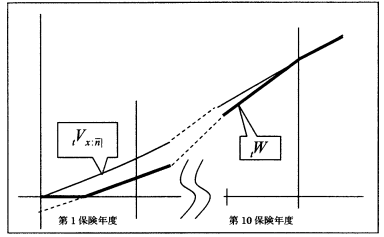
\includegraphics[scale=0.8]{images/ProbH16-1-2-3.png}

\answer{解答}

\begin{itemize}
 \item [1)] 営業保険料申の予定新契約費(年額)が$\frac{\alpha}{\ax**{\endowxn}}$であり、前提②より
$$
F+\frac{\alpha}{10\cdot\ax**{\endowxn}}
=\frac{\alpha}{\ax**{\endowxn}}+\frac{9}{10}\alpha^{*}
\, \, 
\text{従って}
 \, \, 
 \alpha^{*}=\frac{10}{9}F-\frac{\alpha}{\ax**{\endowxn}}
 $$
 \item [2)]
\end{itemize}
 \begin{table}[h]
\begin{tabular}[t]{|c|l|l|l|}
\hline
 \multirow{2}{*}{a)}&\multirow{2}{*}{第1保険年度末} &費差損益 & $\frac{\alpha}{\ax**{\endowxn}}-(F+\frac{\alpha}{10\cdot\ax**{\endowxn}})$\\ \cline{3-4}
 & &解約益 & $\Vx[1]{\endowxn}-_1W = \frac{9}{10}\alpha^{*}=F-\frac{9}{10}\frac{\alpha}{\ax**{\endowxn}}$\\ \hline
 \multirow{2}{*}{b)}&\multirow{2}{*}{第2保険年度末} &費差損益 & $1\frac{\alpha}{\ax**{\endowxn}}-(F+\frac{2\alpha}{10\cdot\ax**{\endowxn}})=\frac{18}{10}\frac{\alpha}{\ax**{\endowxn}}-F$\\ \cline{3-4}
 & &解約益 & $\Vx[2]{\endowxn}-_2W = \frac{8}{10}\alpha^{*}=\frac{8}{9}F-\frac{8}{10}\frac{\alpha}{\ax**{\endowxn}}$\\ \hline
 \multirow{2}{*}{c)}&\multirow{2}{*}{第10保険年度末} &費差損益 & 10$\frac{\alpha}{\ax**{\endowxn}}-(F+\frac{5\alpha}{10\cdot\ax**{\endowxn}})=9.5\frac{\alpha}{\ax**{\endowxn}}-F$\\ \cline{3-4}
 & &解約益 & $\Vx[10]{\endowxn}-_{10}W =0$\\ \hline
\end{tabular}
 \end{table}


\problem{H9 生保1問題 3(3)①}

費差損益、死差損益の影響が少ない貯蓄性商品に関し、解約返戻金支払の増大が予測される状況を挙げよ

\answer{解答}

\begin{enumerate}
 \item 出題の視点
\begin{enumerate}
 \item 出題の趣旨は、費差損益や死差損益等の保険関係バッファーの乏し
い貯蓄性商品について、その商品特性、顧客二一ズ等を踏まえた流動
性リスクの考察と、それらに対するALM的視点からの解約返戻金面
での対応策を問うことにある。
 \item 従って、解答においては、例えば新契約費の未償却部分の回収等の
伝統的な解約返戻金のあり方の視点ではなく、上記の出題趣旨に沿っ
た解答を期待した。
 \item 本間題のみならず、解答に際しては、過去問題の模範解答の丸写し
的な解答ではなく、出題趣旨を十分踏まえた、自己の考え方に基づく
論点の整理、所見を今後とも期待する。
\end{enumerate}
 \item 解答のポイント
\begin{enumerate}
 \item 解約返戻金支払の増大が予想される状況を挙げよ。
\begin{itemize}
 \item 一般的に「 費差損益、死差損益の影響の少ない貯蓄性商品」と言って
も、その商品特性の違いによって、顧客二一ズ・意識が異なってくる
と想定されるため、例えば以下のような切り口での想定し得る商品性
およびそれに対応する顧客二一ズ・意識についての説明を行った上で、
解約返戻金支払の増大が予測される状況を述べる必要があろう...
 \item 一時払 or 平準払
\begin{itemize}
 \item 一時払(養老、個人年金等)については、平準払に比して、より顧客
の金利選好意識・他業態競合商品との利回り比較意識が働くものと考
えられる。また、ALM管理の面から資産とのマッチングを行いやす
いのも一時払であるが、一方、解約時のミスマッチが生じやすいのも
一時払になろう。
 \item 従って、例えば、金利上昇局面において、隣接金融商品との利回り面
での劣位状況が生じた場合には、主として一時払について、解約の増
大、隣接金融商品への預け換え等の状況が想定される。
\end{itemize}
 \item 伝統的商品 or 金利感応型商品等のニューウェイブ商品
\begin{itemize}
 \item 伝統的商品については、無配当保険の場合の価格(予定利率)硬直性、
有配当保険の場合の配当決定方法(年1回、市中金利状況と運用利回
りとのタイムラグ等)により、金利下降局面では相対的な価格優位性
が期待し得るが、逆に、金利上昇局面では相対的に価格面で不利にな
ることが想定される.
 \item 従って、上記と同様に、金利上昇局面等における金利感応度の遅れに
伴う解約の増大、下記のニューウェイブ商品を含めた金利感応度の高
い金融商品への預け換え等の状況が想定される。
 \item 一方、金利感応型商品等のニューウェイブ商品については、その商品
特性によっても異なってくるが、当然、伝統的商品に比べ金利感応度
は高くなるよう商品設計されている、しかしながら、金利感応の仕組
み(新規契約から適用、既契約については固定 or 複数年毎に見直し
等)によっては、金利上昇局面で価格面で不利になることも想定され、
更には、株価連動タイプ商品等では、株価下落局面での顧客の収益確
定ニーズが働くことも考えられる.
 \item もっとも、この問題については、後述のニューウェイブ商品設計にお
ける解約返戻金設定方式による、解約二一ズに対する抑止力、解約時
のミスマッチによる会社損失の回収を図ることにより対応することが
考えられる。
\end{itemize}
 \item 個人向け or 団体向け
\begin{itemize}
 \item 個人向け商品に比して、団体向け商品(団体年金等)については、よ
り顧客のパフォーマンス比較意識が働きやすいものと考えられる(他
業態競合商品も含めた品揃えの多さ、それらとのパフォーマンス比較
による顧客の選別意識の高さ等)
 \item 更には、団体の規模や商品特性・年金制度等の違いによる顧客の意識
の違いも想定される、例えば、大規模団体の方が相対的にパフォーマンス比較
意識が高いものと考えられるし、年金制度を併せて受託しな
い運用契約的色彩が強い契約の方が、相対的にパフォーマンス比較意
識が高いものと考えられる。
 \item 従って、これらパフォーマンス比較・選別意識が高いと想定される団
体顧客については、金利上昇局面のみならず、株価上昇局面等におけ
るトータルパフォーマンス比較において、他業態競合商品とのバフォ
ーマンス劣位状況になると、解約・シェアダウンの増大、よりバフォ
ーマンスの高い提供商品への移行等の状況が想定される,
\end{itemize}
\end{itemize}
\end{enumerate}
 \item 1(以下 ①)を踏まえ、解約返戻金のあり方について所見を述べよ。
\begin{itemize}
 \item 商品設計(区分経理、価格設定への反映等を含む)上の留意点等
\begin{itemize}
 \item ①の商品特性、顧客二ーズ・意識等を踏まえ、商品設計上の留意点、
区分経理(資産区分)の必要性、価格設定への反映のあり方等につい
て説明する必要があろう。
 \item 費差損益、死差損益の影響が少ない貯蓄性商品は、費差損益・死差損益等
のバッファーが期待できないため、負債サイドと対応する資産サ
イドとのミスマッチリスクを生じさせないような対応が必須になる.
 \item 従って、伝統的商品、ニューウェイブ商品の如何を問わず、区分経理
(資産区分)による内部管理は重要であり、商品・負債特性に応じた
運用ポートフォリオ設定・マネージメントを行う必要がある。(例え
ば、一時払(養老)については、国内債券を主体とした満期・償還等
がマッチングした運用ポートフォリオの構築等)
 \item また、解約等の資金流出リスクが想定される商品については、流動性
も考慮した機動的な運用ポートフォリオ対応も必要になろう
 \item これらの区分経理(資産区分)におけるセルフサボーティングを前提
として、価格設定においてもそれらの状況を反映することが用干要であ
る.
 \item 伝統的商品においては、予定利率水準の決定、資産区分運用成果を踏
まえた配当率水準の設定がポイントになるし、ニューウェイブ商品に
ついては、例えば金利感応型商品では、金利感応ルールの決定(新規
契約における設定利率の見直しのタイミング、既契約における見直し
サイクル、見直しルール、最低保証水準の設定等)がポイントになろ
う
\end{itemize}
 \item 上記商品性・資産区分に伴う解約価格への反映のあり方
\begin{itemize}
 \item 上記対応により、契約継続を前提としたミスマッチリスクを回避でき
たとしても、契約途中での解約によるミスマッチリスクは依然残るこ
とになる
 \item 例えば、一時払(養老)において、上記対応により契約継続を前提と
したマッチングが図れたとしても、金利上昇局面での相対的な利回り
低下に伴う解約時には、対応する資産(ここでは主として国内債券)
が含み損を抱えた状況になり、それらを解約価格に反映できないと、
解約ミスマッチリスクとして会社が損失を被る懸念がある.
 \item 従って、基本的な対応としては、区分経理(資産区分)で管理する負
債対応資産の時価資産相当額を解約価格に反映させる考え方が重要に
なってくる。
 \item これらの基本的なスタンスの中で、以下の論点を踏まえた所見を期待
する
 \item 解約価格への反映方式〜時価資産価値の解約価格へのダイレクトな反
映(MVA)、ミスマッチリスク期待値のフォーミュラ化等による解
約控除率の設定
 \item 顧客の理解度・許容度・説明〜個人向け or 団体向け等の顧客理解度・
許容度等の違いによる解約価格への反映方式の決定、契約時における
顧客宛説明の徹底
 \item 区分経理(資産区分)状況のディスクロージャー〜MVA方式等を採
周する場合の区分経理(資産区分)状況のディスクロ』ジャーの必要
性 等
\end{itemize}
\end{itemize}
\end{enumerate}
\end{document} 